%% ----------------------------------------------------------------
\chapter{Design Approaches Considered}
%% ----------------------------------------------------------------

\section{Payload Image Capture}

\section{Camera Module}
\label{sec:John_options}

A range of different camera modules were researched and considered for use in the project. It was decided early on in the project that camera modules would be used rather than attempting to interface with standard digital cameras.

\subsection{Approach: USB Camera}
\label{sec:USB_option}
Many USB webcams are available for purchase and this was considered as a possibly approach.

Advantages:
      \begin{itemize}
         \item Low cost of typically around £15
         \item High resolution of typically 1 to 3 Megapixels
		 \item Small size
		 \item Cabling included so can be easily positioned in the UAV
     \end{itemize}

Disadvantages:
     \begin{itemize}
        \item Difficult to communicate with
        \item Requires USB host device
		\item High resolution means longer transfer times
     \end{itemize}

This approach was ruled out because of the difficulty in communicating with this camera type. In order to communicate with a USB camera a USB host is required and as the process is usually fairly complex a driver is normally used. This is extremely difficult to implement on a device compact enough for use in this project.

\subsection{Approach: Analogue Camera}
\label{sec:Analog_option}
Camera modules with analogue composite outputs are available, usually for cctv or surveilence purposes, and were also considered as an approach.

Advantages:
      \begin{itemize}
         \item Range of resolutions available
		 \item Small size
     \end{itemize}

Disadvantages:
     \begin{itemize}
        \item Awkward to communicate with
        \item Require case and cabling for placement in UAV
		\item Can be expensive at up to around £80
		\item Often video rather than still cameras
		\item Often black and white rather than colour
     \end{itemize}

This approach was ruled out because of the additional complexity required in converting from analogue to digital whilst maintaining all the information in the image, that would be required to send an image from a camera of this type through a microprocessor.

\subsection{Approach: Serial Camera}
\label{sec:Serial_option}
Some camera modules are available with UART rather than USB serial communications and these to were considered as an approach.

Advantages:
      \begin{itemize}
		 \item Easy to communicate with
         \item Range of resolutions available
		 \item Small size
		 \item Well documented
     \end{itemize}

Disadvantages:
     \begin{itemize}
        \item Require case and cabling for placement in UAV
		\item moderately expensive at around £40
     \end{itemize}

This was the approach that was chosen as the ability to communicate via UART combined with the good documentation should allow for control to be established fastest with this camera type.


\section{Local Image Storage}
\label{sec:local_storage}

With a maximum image size of $640\times480$ pixels, an uncompressed JPEG 
image's file size would be approximately 900kB.
This is greater than the internal memory on the ATmega168, ATmega328 and 
ATmega644 (1KiB, 2KiB, and 4KiB respectively) microprocessors that were used 
during development of this project, therefore it cannot be guaranteed that a 
complete single image can be stored locally, without adding some extra memory.
\\
The advantages of being able to store a full image locally are:
\begin{itemize}
\item Would allow all original images taken during flight to be viewed once 
the UAV has been landed.
\item Would make the implementation of automatic repeat requests (resending of 
any corrupted payload -$>$ ground station packets) much easier.
\item Customer mentioned that currently, customers take images with their 
retrofitted cameras, but store the images locally instead of wirelessly 
transmitting them. Keeping the functionality to store all images taken 
on-board and then plug something into the ground station to view these once 
the UAV has been landed would be desirable, but not essential (hence why this 
is not mentioned in the specification).
\end{itemize}

The disadvantages:
\begin{itemize}
\item The material cost of the payload (in both component cost and PCB area) 
would be increased.
\item Addition of an extra component increases the project's complexity.
\end{itemize}

\subsection{Approach: Flash Chip}

One option considered was the implementation of an external flash memory chip 
(for evaluation purposes, the 4Mbit AMIC A25L040-F was purchased)

Advantages:
\begin{itemize}
\item Non-volatile memory. Allows data to be retained even if power to the payload module is cut off.
\item Excellent data integrity: ~100000 Write/Erase cycles, and $>$10 years data retention.
\item Relatively good operating current of ~20mA makes it suitable for battery-powered application.
\end{itemize}

Disadvantages:
\begin{itemize}
\item Chips that contain a significant amount of memory storage (e.g. 1Gbit 
and above), come in packages that are awkward to prototype (BGA, TSOP)
\item Interfacing this type of device with a PC would require a similar amount 
of work to the ground station software.
\item Non-standard interface. The command set for the 4Mbit device is not the 
same as for a 1Gbit device.
\end{itemize}



\subsection{Approach: SD Card}

This is essentially the same as the flash chip above, but with an additional controller chip, and packaged in a standard case.

Advantages:
\begin{itemize}
\item Non-volatile memory. Allows data to be retained even if power to the payload module is cut off.
\item Same data integrity as for the above item.
\item Getting image data from the card would be as trivial as removing the 
card from the payload and inserting it into the ground station laptop. SD card 
readers are cheap, and ubiquitous.
\item Good value for money, when compared to price-per-Mbit of the other two 
options under consideration. (For example, a 2GB microSD card (including 
microSD -$>$ SD adapter) from Amazon costs ~£4.
\end{itemize}

Disadvantages:
\begin{itemize}
\item Open source libraries can only make use of an SD card's SPI Bus
interface, not the quicker (but patent-covered) four-bit SD bus.
\item Only standard SD cards may be used, not the more recent SDHC or SDXC 
cards, which are increasingly popular.
\end{itemize}

\subsection{Approach: SRAM}

SRAM was considered as a possible option as we had all used this before.

Advantages:
\begin{itemize}
\item We have previous experience of interfacing these with AVRs from a 
second-year lab, 
\item This type of memory performs read/write operations much quicker than 
the other two options.
\item Very low operating current of ~10mA makes it suitable for this battery-powered application.
\end{itemize}

Disadvantages:
\begin{itemize}
\item Standard SRAM is volatile, so data is prone to being lost if the payload 
module power is lost, or the payload module is reset. (While non-volatile SRAM 
does exist, it is much more expensive per Mbit (~£18/Mbit) than the other 
options under consideration.)
\item Comparatively expensive
\item Communication with the device requires connection to all data, address 
and control pins (or implementation of shift registers with the same desired 
effect), this would require more board space. (The other two devices can 
communicate via an SPI bus, a four wire connection)
\end{itemize}

\section{Payload Controller Hardware}
The hardware used to implement the payload controller is an important consideration.

The exact requirements for this module depend on other design decisions made, such as the method used to interface with the camera module. However there are a certain fixed set of requirements derived from the specification:

\begin{itemize}
\item The module must communicate with the autopilot over an asynchronous RS-485 serial connection at 38.4 kBaud. This suggests that the module should have access to some form of UART.
\end{itemize}

Additional requirements depend on other design decisions:

\begin{itemize}
\item \emph{Camera communication:} Using a serial camera would mean the controller requiring access to another UART, while using a USB camera leaves the camera needing access to a USB host interface. Similarly using an analogue camera would mean either the controller be capable of digitising the camera data itself or having a method of interfacing with an external digitiser.
 
\item \emph{Image buffering:} Most embedded systems do not have enough RAM or Flash to store a reasonable sized image on onboard memory. As described in section \ref{sec:local_storage}, there are a number of approaches worth considering for externally buffering an input image, however these do require the controller to have an interface with which to communicate with the external memory. 

\item \emph{Progressive JPEG Manipulation:} Section \ref{sec:implementation_progressive_jpeg} details several ways progressive JPEG manipulation could be tackled. Depending on the design choice taken this could influence the requirements of the controller substantially. Examples of such requirements could be: extra processing power, fast access to memory or FFT or DCT libraries being available for the device.
\end{itemize}

\subsection{Approach: Digital Signal Processor (DSP) Development Board}
An appropriate Digital Signal Processor (DSP) development board would provide fast digital signal processing capabilities to the controller. This would be especially useful for the situations mentioned in section \ref{sec:implementation_progressive_jpeg}.

Since DSP chips tend to be specialist devices they are usually difficult to set up or program without first experimenting with the design using a development board - a special board designed with experimentation and product development in mind. Ideally a development board would be used for initial development of the system with a integrated PCB being developed later on to allow the DSP to be used on its own.

Advantages:
\begin{itemize}
\item DSPs often have very good analogue to digital conversion built in as standard. If an analogue camera is used (as discussed in section \ref{sec:Analog_option}) a DSP may provide the necessary fast ADC without any extra components.

\item Libraries for tasks such Fast Fourier Transforms or other signal and image processing related applications are often readily available for DSP chips. For some methods of performing progressive JPEG manipulation (see section \ref{sec:implementation_progressive_jpeg}) this could be useful.

\item Large number of miscellaneous signal processing related hardware features built in which could be useful in as-yet unforeseen circumstances.
\end{itemize}

Disadvantages:
\begin{itemize}
\item DSP chips are often complex and may require significant work to produce a system running without a development board.

\item DSP development boards often cannot be used effectively in a final version of a project due to size and power constraints.

\item There is a steep learning curve to using these devices and the group has very little experience with them.
\end{itemize}


DSP boards are a specialist tool, which could be especially useful - if not required - if implementing certain image processing algorithms such as some of those detailed in section  \ref{sec:implementation_progressive_jpeg}|. The downside of this is a more complex overall system.

\subsection{Approach: Atmel 8-bit AVR}
\label{sec:desappr:avr}
The Atmel 8-bit AVR family is a well-known set of low cost, single chip microcontrollers. Specific parameters taken from \cite{megaAVR_parameters}.

Advantages:
\begin{itemize}
\item All members of our group have had experience working with AVR chips.

\item Programming and debugging devices are readily available to us.

\item Creating stand-alone systems easy: no need for large amounts of additional components.

\item Commonly used devices mean large community built around the device family meaning support and additional libraries are more likely to be available.

\item Some initial payload code available to us already implemented on a AVR, see section \ref{sec:team_resources}.

\item Large range of different devices which work with the same programming tools and minimal code changes available.

\item Many through-hole versions of the devices are available, making prototyping significantly easier (and cheaper, due to lack of need for breakout boards) than using surface mount components.
\end{itemize}

Disadvantages:
\begin{itemize}
\item Most 8-bit AVR devices are reasonably low speed (20MHz maximum), meaning they could be unsuitable for heavy calculations such as image processing.

\item 8-bit AVRs do not have floating point processing units, making some image processing tasks much slower to complete on an AVR.

\item Less communication options than some other, more complex, devices. This limits the number of peripheral devices that can be connected to the controller at once, and so may reduce flexibility.

\item Limited RAM available on the commonly used devices which are available in through-hole format. A common amount of RAM for a larger through-hole AVR is 4 kbytes.

\item The smaller, cheaper, devices have reasonably limited program memory, with 64 kbytes being a typical amount for a larger through-hole device. This could be a problem if implementing large amounts of code or using significant numbers of lookup tables for example.
\end{itemize}
	
AVRs are robust, widely used, general purpose microcontrollers. The large community surrounding them is a particular advantage, as it means many libraries and development boards are available for the devices. Our previous experience with the devices is also a key advantage, although it is important to be aware of the devices limits.


\subsection{Approach: Atmel 8-bit AVR with Arduino Prototyping Platform}
\label{sec:appr_considered_arduino}

The Arduino platform is a low cost, open-source development platform for the Atmel AVR microcontroller family. The latest versions of the development platform consists of an ATMega328 microcontroller along with voltage regulators, inbuilt USB programmer and serial interface and 16MHz crystal. A software library for the device provides a wrapper around many of the complexities of the AVR platform, allowing more rapid development to be possible than with a pure AVR. A simple IDE is used to program the device and a wide range of extra libraries are available which target the platform. The physical platform is designed to be easily extended using expansion boards called `shields'.

The advantages and disadvantages of the Atmel 8-bit AVRs mentioned in section \ref{sec:desappr:avr} also apply.

Advantages:
\begin{itemize}
\item Just an ATMega328 `under the hood' meaning that the additional power of the chip can be leveraged if needed.

\item Many common tasks such as setting the baud rate of the serial link are made very simple by the Arduino libraries, meaning development time can be spent working on more challenging features.

\item Very widely used by hobbyists, meaning a large number of open-source libraries are available for the platform.

\item Platform is easily available meaning others should more easily be able to replicate project. Widely used platform means plenty of support is available for others wishing to re-implement this project.

\item Since only a `shield' expansion board would need to be manufactured this would cut time otherwise spent designing and making board for AVR.
\end{itemize}

Disadvantages:
\begin{itemize}
\item Using the Arduino libraries means a certain amount of unused overhead is likely.

\item The Arduino libraries hide much of the complexity of the device. This can mean advanced features are hidden or not exposed, negating some of the advantages of the library when advanced features are needed.

\item Design would consist of two parts: Arduino board and expansion `shield'. This could reduce durability and increase size.
\end{itemize}

Using an Arduino has the advantage of speeding up development at the beginning of the project. The large number of libraries built for the Arduino is another key advantage, as is the ease of re-implementation.

\subsection{Approach Chosen}
We chose to use an Atmel 8-bit AVR as the platform for our implementation of the payload controller. Our main reason for choosing this platform is because we already have experience in using this microcontroller, meaning less time to develop and 
test the system over a DSP based solution. Another key reason was the ease of implementing AVR based systems as 
stand-alone boards.

\section{Communication between Payload Controller and Ground Station}
One of the key tasks of the payload controller is to communicate with the Ground Station via the Autopilots 38.4 kBaud serial link. In order to fulfil the specification the payload controller must be capable of receiving messages/commands sent from the Ground Station image viewer software (see section \ref{chap:implementation_ground_station}) through the autopilot link, as well as be capable of sending data to the Ground Station Image Viewer.

The autopilot provides a number of ways to communicate between a payload module and ground station software. The Ground Station software provided to us allows a `packet' of data to be sent to a payload module by executing the command shown below

Another method of communication is via the use of shared memory. Each registered payload module is assigned a set of shared memory which can be read and set by the payload module and the ground station software. This could be used to implement two-way communications between the two subsystems.

The design approaches taken regarding this communication from the perspective of the Ground Station Image Viewer software is discussed in section \ref{chap:implementation_ground_station}.

\subsection{Approach: Shared Memory for Both Directions}
One possible way of producing two-way communications would involve two sets of shared memory: one for ground station to payload messages and another for payload to ground station messages. Both the payload and the autopilot would need to poll the shared memory to check for new messages.

%Advantages:
%\begin{itemize}
%\item 
%\end{itemize}

Disadvantages:
\begin{itemize}
\item The payload must access shared memory by sending a command to request a copy of its contents to be sent via the payload-autopilot serial link. This extra overhead would slow down communications.
\end{itemize}


\subsection{Approach: Send Bytes Command and Shared Memory}
The send bytes command could be used to send messages from the Ground Station to the payload, with shared memory being set by the payload to send messages back from the payload to the Ground Station.

Advantages:
\begin{itemize}
\item No overhead needed to get messages on the payload, they are sent directly from the autopilot to the payload, no polling needed.
\end{itemize}

%Disadvantages:
%\begin{itemize}
%\item Error coding??
%\end{itemize}

\subsection{Approach Chosen: Send Bytes Command and Shared Memory}
Using shared memory for one direction and send bytes for the other seemed like a sensible choice due to the lower overhead needed.


\section{Image Manipulation (ms)}
\label{sec:progressiveimagedisplay}

The design of the progressive image
display system to be implemented on the
payload and the ground station required some
important decisions to be made before 
development could begin. This included
the type of image file which would be
manipulated, how the image sent from the camera on 
the UAV would be accessed,
and the method of storing the data
and sending it to the ground station.

\subsection{Image File to Manipulate}

The first design decision was to choose the type of image 
file which would be the most practical to work with given
the properties of the camera and the
capabilities of the payload software. Factors taken into
account in this decision include compatibility with the 
camera module as well as efficiency in the compression
process.

\subsubsection{Approach: Custom Raw Image Manipulation}

This approach involves using the custom image 
manipulation algorithm as specified 
in section \ref{Custom_comp_research}.

Advantages:
\begin{itemize}
	\item Would be able to handle the images
		given by the camera regardless of the format
		the camera saves the image.
	\item Avoids quantization to allow 
		for lossless compression: No information is
		lost when the image is 
		compressed and decompressed.
	\item Uses a simple, reliable, and easy to 
		understand image compression technique
		(Discrete Cosine Transform)
	\item Can more easily create a progressive
		display of the image due to having less
		information to decode.
\end{itemize}

Disadvantages:
\begin{itemize}
	\item Restricted to decoding raw images; 
		cannot deal with JPEG images.
	\item Does not compress the image as 
		efficiently as more advanced 
		image compression techniques.
\end{itemize}

\subsubsection{Approach: JPEG File Manipulation}

This approach involves manipulating JPEG standard image 
files instead of raw image files. This requires the
microcontroller to work around the compression offered
by the JPEG file standard (see section \ref{jpeg_image_compression}).

Advantages:
\begin{itemize}
	\item Compatible with most standard
		camera outputs.
	\item Takes advantage of the reliable and
		efficient JPEG compression algorithm.
	\item Uses quantization to allow for a greater
		degree of image compression.
\end{itemize}

Disadvantages:
\begin{itemize}
	\item Compression is lossy: image loses 
		more and more information 
		each time it is compressed 
		(saved and opened).
	\item Requires more sophisticated and complex
		decompression algorithms.
	\item Requires more background research to
		understand and manipulate.
\end{itemize}

\subsubsection{Chosen Approach: JPEG Manipulation}

Before the camera was agreed upon, work began on the
custom raw image compression algorithm. This
allowed us to get a good idea of how the progressive
display of the image would work in the final product.
However, when the camera was chosen, it's output
was restricted to JPEG image files. Therefore, JPEG 
file manipulation was chosen in order to adapt to
the hardware given.

\subsection{JPEG File Manipulation}
\label{sec:jpegmanipulation}

This section weighs the decision of implementing a 
form of custom JPEG image manipulation to allow the 
image to be displayed progressively, as requested by the customer.

\subsubsection{Approach: Custom JPEG Manipulation}

This design approach details the choice to code an algorithm which 
would modify the image received from the camera in order to 
display it progressively. Ideally, this would send an extremely low 
detail image to the ground station which would progressively improve 
while more information is sent from the camera by implementing 
the higher frequency components of the image.

Advantages:
\begin{itemize}
	\item Allows an image to be sent and 
                     be manually evaluated sooner.
	\item Allows the user to cancel images which begin to show 
		unwanted information, saving processing time.
	\item Can possibly allow the image information to be 
		optimized, sending only the 
		information necessary for display.
\end{itemize}

Disadvantages:
\begin{itemize}
	\item Requires effort and time, including research into 
		the manipulation of the JPEG format.
	\item Benefit is minimal if the sending a simple image 
		is already very quick.
\end{itemize}

\subsubsection{Approach: Standard JPEG Transfer}

This design approach simply displays the JPEG image from 
the camera as it is received. 

Advantages:
\begin{itemize}
	\item Requires little to no effort 
		(already done by default).
	\item All the metadata of the image is kept unchanged.
\end{itemize}

Disadvantages:
\begin{itemize}
	\item Takes time to send all the image data to the ground station.
	\item During the transfer period, state of image is unknown and 
		can be wasted if image is undesirable.
	\item Image sends all the metadata, including 
		metadata which can be ignored.
\end{itemize}

\subsubsection{Chosen Approach: Custom JPEG Manipulation}

Prior to knowing the exact speed it would take to send 
an image from the camera to the ground station, 
it was decided that custom JPEG manipulation would optimize 
the image further and help reach the target time specified (3 minutes). 
Therefore, tasks concerning the custom manipulation of 
the JPEG image were planned and worked on 
at the beginning of the project. 
However, when a working module was constructed, the time needed to 
send the image was already well within the time specified. 
Because this was the primary advantage of the 
custom JPEG manipulation process, 
the task's priority was dropped accordingly.

\subsection{JPEG Data Access}

One of the biggest choices to make concerning the 
image manipulation software to be implemented on the AVR was 
how it would  access the JPEG image data coming from the camera. 
The two methods considered are studied below:

\subsubsection{Approach: Static Access}

This method of accessing the image data involves storing 
the JPEG image data into memory and 
having the AVR read the JPEG data as if it were a data array. 

Advantages:
\begin{itemize}
	\item Easier to provide progressive scanning of the 
		image due to possessing the entire 
		entropy-encoded image data. It is easier to 
		read the whole image rather than 
		have the data coming in at a certain rate on the AVR.
		This would allow the AVR to have more options on
		the order of the image data to send.
	\item Much fewer calls to the JPEG byte stream. 
		This allows the extractor to obtain all the 
		information faster from the moment it is called.
	\item Only one instance of memory allocation at the very beginning. 
		This prevents the code from crashing due to insufficient 
		memory in the middle of the information 
		extraction process and wasting time.
\end{itemize}

Disadvantages:
\begin{itemize}
	\item Very memory intensive: requires 
		storing the entire image in memory 
		before being called due to the variable
		size of the JPEG file and its components.
	\item Delayed by image storage.
		Although there is only one call to the 
		image data, it must wait until the entire 
		input string is stored before 
		any action can be taken safely.
	\item A lot of wasted memory. 
		Not all the information 
		from the image is needed for the 
		progressive JPEG manipulation.
\end{itemize}

\subsubsection{Approach: Dynamic Access}

This method of accessing the image data 
involves using a class to read in one byte 
from the image data stream at a time.

Advantages:
\begin{itemize}
	\item More efficient for memory 
		space overall. No need to store 
		the entire image at once.
	\item Allows more efficient use of memory. 
		The AVR only saves and sends the 
		information that the ground station will use.
\end{itemize}

Disadvantages:
\begin{itemize}
	\item More difficult to use progressive scanning. 
		Entropy-encoded data must be stored fully 
		before progressive scanning can occur.
	\item Delayed by multiple read calls to the JPEG data. A 
		read call must be made for each 
		byte of the JPEG data stream.
	\item Memory allocated dynamically. 
		More vulnerable to insufficient memory 
		crashes during the extraction process.
\end{itemize}

\subsubsection{Chosen Approach: Dynamic Access}

The dynamic form of data accessing was preferred 
due to the memory constraints imposed on the device.

\subsection{Entropy-Encoded Data Storage}

Another major decision to make was the method of 
storing the entropy-encoded image data of the JPEG file, 
which is divided into chrominance pixels made up of 
3 different components.(See section 
\ref{sec:colour_space_conversion} for
more information on chrominance pixels.)

\subsubsection{Approach: Store As Chrominance Pixels}

This method stores the chrominance pixels in 
the image one by one. 
The data is stored in a linked list of chrominance pixels, 
containing a certain number of Y values and 
one pair of Cb and Cr values.

Advantages:
\begin{itemize}
	\item Makes the YCbCr colour modelling method 
		more obvious. 
		This method intuitively partitions the 
		encoded image data using the YCbCr convention.
	\item Requires little data manipulation. 
		Structures are made as input stream is read in, 
		one at a time.
	\item Comprehensive memory allocation. 
		Allocates the appropriate memory for 
		one chrominance pixel as needed.
\end{itemize}

Disadvantages:
\begin{itemize}
	\item Encoded image data becomes more 
		difficult to apply progressive scans to.
	\item No spatial information is stored. 
		Data is stored as a linear list of chrominance 
		pixels instead of a table representing the image.
	\item Memory must be allocated dynamically. 
		More vulnerable to insufficient memory 
		crashes during the extraction process.
\end{itemize}

\subsubsection{Approach: Store Components Seperately}

This method of accessing the image data involves 
storing the three components Y, Cb, and Cr into tables.

Advantages:
\begin{itemize}
	\item Makes progressive scanning easier. 
		The three components can be selected individually.
	\item Information can be stored in a table to 
		represent the image spatially.
	\item Memory can be allocated either 
		dynamically or prior to the read process.
\end{itemize}

Disadvantages:
\begin{itemize}
	\item Requires more manipulation of the 
		entropy-encoded image data as it is read in. 
		Components must be monitored to not 
		lose chrominance pixel grouping.
	\item Chrominance information must be stored either 
		unintuitive (a smaller table than the image) or 
		inefficiently (an image sized table with empty values).
	\item Generally more difficult to monitor the information stored.
\end{itemize}

\subsubsection{Chosen Approach: Store As Chrominance Pixels}

The entropy-encoded data will be stored as chrominance 
pixels for the sake of clarity. 
It is also a method which could be coded more easily 
than separate component storage. 
This allowed the AVR to work with the progressive 
JPEG encoder sooner to avoid the task from overrunning.

\section{Ground Station Image Viewer}
The UAV ground receiver is a USB-compatible device. USB device driver has been developed by the customer’s so the hardware can be accessed by ground station software, and other applications. The USB is active when the host ask for a data. The host is the computer network which the UAV connect to. The data in its queue until the host ask for the data. The device listen to its address and request for its specific address. The TCP/IP connection between the port and the GUI must be implemented without any hesitation from the user. The data transmitted from the devices stream data to PC for further data processing (image processing).  The customer’s software is in user mode, where the programmer does not have the right to access directly to the hard ware in protected operating systems. However, there is some code that allow the programmer to communicate with the payload via the ground station software.

The operating system we do the software development and testing is Window7. An operating system has drivers for whatever hardware the end user chooses to populate the system with. The Microsoft Visual Studio 2010 provides a framework for drivers that operate in the operating system. Upon the final stage of the GUI, the software code runs either in user mode or in kernel mode \cite{tsuiK}. This allows a different level of privilege in accessing memory and other system resources. 
\subsection{GUI development process} 
\flushleft
\begin{enumerate}


\item	The most important process of GUI development is to understand what does the customer wants. 

\item	The hardware and software specification have to be determined.
 
\item	Make a GUI design decision

\item Develop a smaller program in order to make the testing easy and less time consuming. 

\item	Learn the .NET class that can support the connection to TCP/IP, and communication between host and device

\item	Use GUI to link to the customer’s software to access the software

\item	Distribute the GUI
\end{enumerate}

\subsection{Approach: Initial Design of GUI}
The GUI design decision based on the specification on what feature does the customer’s want. The user for our application is assumed to have a limited programming experience, so the program will be implemented so it is simple understand. Figure~\ref{ini_GUI} show the first brainstorm view of the GUI. 

The user interface has a picture box. When the user push a ‘Get Picture’ button, the picture box will display the picture taken from the UAV. During the downloading process, the application should keep running so the cancel button can be used. The gallery button will link to another page which will be the collection of all the image taken. The left and right button can navigate the picture box to view an earlier picture or later picture. The Cancel button cancel the receiving image, therefore the corrupted picture will not be downloaded. The user mode of the application can access only the main feature such as take picture, change directory, and cancel download picture.  It allows the user to choose the resolution and picture type (RAW or JPEG) to transmitted from the UAV to the ground station. But the user doesn't have access to changing the command, changing the receiving data, and any interaction with the UAV because of safety and avoid of any errors. 
\begin{figure}[!hbtp]
\begin{center}
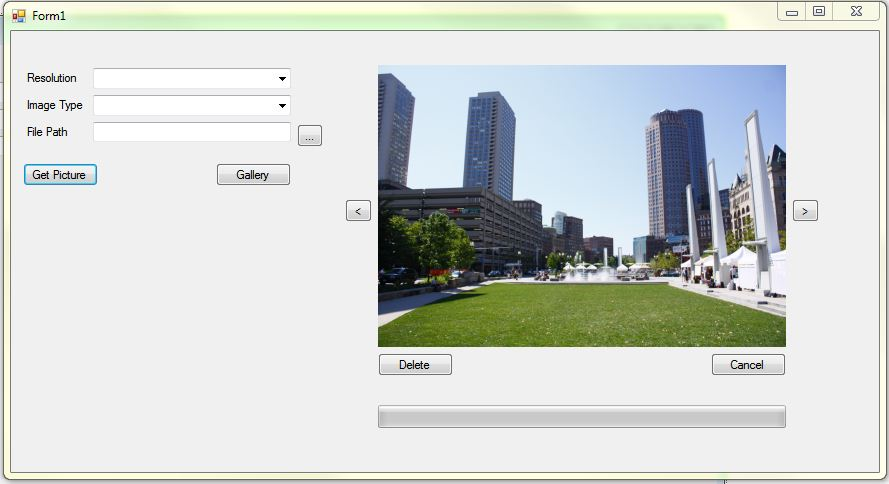
\includegraphics[scale=0.7]{figures/initialGUI.png} 
\end{center}
\caption{The initial design of GUI\label{ini_GUI}}
\end{figure}

\subsubsection{Initial Class Diagram}

Figure~\ref{ini_Class} shows initial design of classes to implement. The \texttt{JPEGFileReader} Class is use for decoding the JPEG file. The decoding method is in the plan of the final program because the image take a long time to download. So, if a  The method is that in the JPEG file, there are headers. In order to make the image progressively better, these header must be extracted. The method commandCheck use check each byte of the image for a \texttt{0XFF} value. For any JPEG file, 0XFF is the start of the header of the JPEG image. The huffman table and quantization table can transform from the byte value. 
\begin{center}
\begin{figure}[!hbtp]
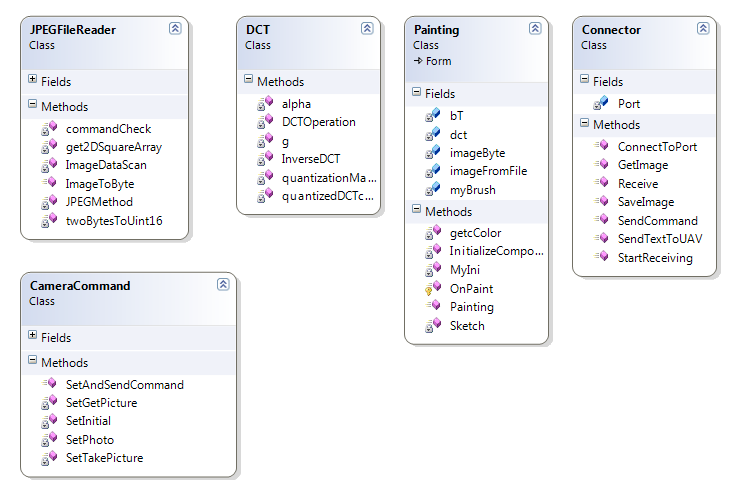
\includegraphics[width=150mm,height=100mm]{figures/initialClassDiagram.png} 
\caption{The initial design of GUI classes\label{ini_Class}}
\end{figure}
\end{center}
DCT has many math operation and equation which have to be implemented on the image viewer program. This include discrete cosine transform, and inverse discrete cosine transform. The inverse DCT for encoding:

\begin{equation}
f_{xy}=\sum_{u=0}^7\sum_{v=0}^7 \alpha(u) \alpha(v) F_{u,v} \cos\Big[\dfrac{\pi}{8}(x+\dfrac{1}{2})u\Big]\cos\Big[\dfrac{\pi}{8}(y+\dfrac{1}{2})v\Big]
\end{equation}

$x$ is the pixel row, for the integer $0< x< 8$

$y$ is the pixel column, for the integer $0< x< 8$

$\alpha(u)$ is a normalizing scale factor

$F_{u,v}$ is the reconstructed approximate coefficient at coordinates $(u,v)$
 
$f_{x,y}$ is the reconstructed pixel at coordinates $(x,y)$

This complicated function should implement in the ground station because if the picture is encoded in the compressed way, the ground station must be able to extract it. In the end, we have to determine whether is it faster to display image normally, or to do encoding/decoding JPEG file. The another downside of this method is that there are many encoding resource which work perfectly, but because of this is long and complex, it might cause some error and time consuming.
The painting class is supported by the DCT class. The intention of this class is to display an encoded image point by point on the picture box.By this method, the pictureBox can display an image at the first pixel.
The \texttt{CameraCommand} class design for send the data from the ground station to the camera. The idea is that make the camera sync with the payload by using the ground command. \texttt{SetAndSendCommand} use for set the byte command and then send it to the payload via the Console port. \texttt{SetGetPicture,SetInitial, SetPhoto, and SetTakePicture} methods are use for setting the correct byte in order to send the byte by using \texttt{SetAndSendCommand} class.




\subsubsection{Use Case Diagram}

Figure~\ref{GUI_useCase} shows a possible user action on the program. The user can save, open and delete any jpeg image from the computer. The program can also detect the corrupted image and ask the user to delete it. The user has an option to connect to the UAV. This is incase of the UAV is not connected properly. The most important function is get picture from the UAV camera. This will send and receive complex command which will be described. The internal program will process the byte and display the information as image onto the pictureBox. The user will then have an option to save the image and close the program.
\begin{figure}[!hbtp]
\begin{center}
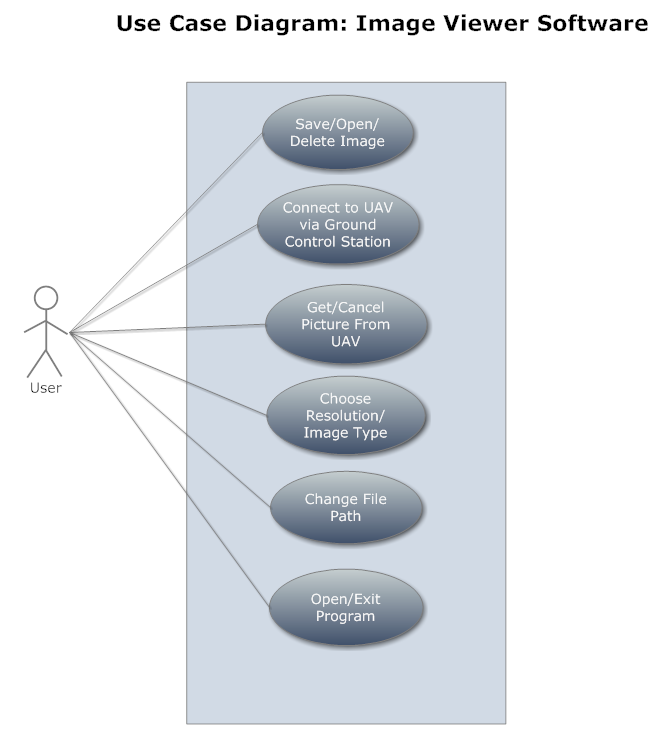
\includegraphics[scale=0.6]{figures/userCase.PNG} 
\end{center}
\caption{Use case diagram of the GUI\label{GUI_useCase}}
\end{figure}



\subsection{Approach: Different C\# .NET Classes}
The C\# language on Microsoft Visual Basic Studio is a development environment for creating our Ground Station Image Viewer application. Choosing the right class to connect to the port helps the developer save time to program the application. The class should be able to connect to the UAV port and it must be able to send both byte and string command and receive bytes camera data from the UAV.  The C\# program has two .NET classes that can connect to port. They are SerialPort Class and Socket Class. 
\subsubsection{SerialPort Class}
The System.IO.Ports namespace contains classes for controlling serial ports. The SerialPort class is the most important one.It has ability to synchronous and event-driven I/O, access to pin and break states, and access to serial driver properties\cite{peak_netFrame}. It can change the port properties such as the stop bit, parity bit, baud rate, etc. It has handshake function that communicate to the port and report if the data or token was received successfully.
By using this class, the COM port setting has to be memorized which will be simple to load and saves from/to disk.In the process both public and private fields of the object and the name are converted to a stream of bytes.

\begin{lstlisting}[caption=Serial Port class connection\, read and write method, label=serialPortconn]
SerialPort( portName, baudRate, parity bit, dataBits, StopBits ) 
SerialPort.Read(Char(),Int32,Int32);
SerialPort.Write(Char(), Int32, Int32)	;
\end{lstlisting}

The advantage of using this class is that the port can change baud rate, handshaking, parity bit, and stop bit. It has an ability to change the internal structure of signal of hardware. The class has a read and writes methods which connection with TCP/IP is possible.
However, the implementation of the class has many unnecessary set up and the code will be very long and can cause error, and it is not possible to reprogram the UAV.
Write() is a SerialPort's public method is use to send data of bytes to an output buffer at the specified offset, it writes a specified number of characters to the serial port using data from a buffer.
Reads method read a number of bytes from the SerialPort input buffer and writes those bytes into a byte array at the specified offset.

If the UAV baud rate is different from the program baud rate, the error will occur.
The parity bit, and end bit and baud rate have to be set up in order to connect to the port, but these set up in UAV already.
\subsubsection{Socket Class}
The Socket is more programmer friendly, robust and a high level connection class. The socket class is use to send and receive data, in similar method as an open file allows an application to read and write data to stable storage.  It also makes a simple handshaking between the client and server machines. It can connect to multi clients, which this is necessary for a multi-port which we are using. The program can easily connect to the port by using the method in Listing\ref{socketClasscrs} .
This method takes the baud rate and parity bit configuration from the UAV so the setup is the same. This class sends and array of bytes to the console port and to the data stream port and receive data from the port by code in Listing\ref{socketClasscrs}.

\begin{lstlisting}[caption=Socket class connect receive and send method,label=socketClasscrs]
Connect (String host name,Int32 port number)
Send(byte[] command, Int32 length, SocketFlags)
Receive(byte[] data, Int32 length, SocketFlags)
\end{lstlisting}

\section{Physical Implementation}

Our specification states that the final module delivered to the customer 
should be on PCB, if time permits. 
	
\subsection{Power Source}

\subsubsection{Approach: Battery Powered}

\subsubsection{Approach: Autopilot Powered}

